\documentclass[a4paper,10pt,twoside,openany]{book}

\usepackage[lang=hebrew]{maths}
\usepackage{hebrewdoc}
\usepackage{stylish}
\usepackage{lipsum}
\let\bs\blacksquare

%TIKZSETS
\tikzset{
    labl/.style={anchor=south, rotate=90, inner sep=.5mm}
}

\title{סיכומי הרצאות בתורת מורס \\ \large{אביב 2021, הטכניון}}
\author{הרצאותיו של מיכאל חנבסקי \\ \large סוכמו על ידי אלעד צורני}
\date{\today}

\begin{document}
\frontmatter
\frontpage{cover}{0.8\textwidth}{חלקים שקולים הומוטופית של הטורוס.}
\tableofcontents
\countlectures
\newpage

\chapter*{הקדמה}
\addcontentsline{toc}{chapter}{הקדמה} \markboth{הקדמה}{}

\section*{הבהרה}
\addcontentsline{toc}{section}{הבהרה} %\markboth{Technicalities}{}

סיכומי הרצאות אלו אינם רשמיים ולכן אין
\emph{כל הבטחה}
כי החומר המוקלד הינו בהתאמה כלשהי עם דרישות הקורס, או שהינו חסר טעויות.
\\
להיפך, ודאי ישנן טעויות בסיכום! אעריך אם הערות ותיקונים ישלחו אלי בכתובת דוא"ל
\textenglish{\href{mailto:tzorani.elad@gmail.com}{tzorani.elad@gmail.com}}.\\
אלעד צורני.

\section*{ספרות מומלצת.}
\addcontentsline{toc}{section}{ספרות מומלצת} %\markboth{Course Literature}{}

הספרות המומלצת עבור הקורס הינה כדלהלן.

\begin{english}
\begin{description}
\item[J. Milnor:] Morse Theory

\item[A. Banyaga, D. Hurtubise:] Lectures on Morse Homology

\item[M. Audin, M. Damian:] Morse Theory and Floer Homology
\end{description}
\end{english}

\section*{ציון}
הציון בקורס ינתן עבור מבחן בית שעשוי (ועשוי לא) לכלול מעבר בעל פה על הפתרונות.

\section*{דרישות קדם}

דרישת הקדם לקורס היא יריעות דיפרנציאביליות. היכרות עם טופולוגיה אלגברית מועילה אך אינה חיונית.

\mainmatter

\chapter{מבוא}
\section{מוטיבציה}

\begin{example}

\begin{figure}
\centering
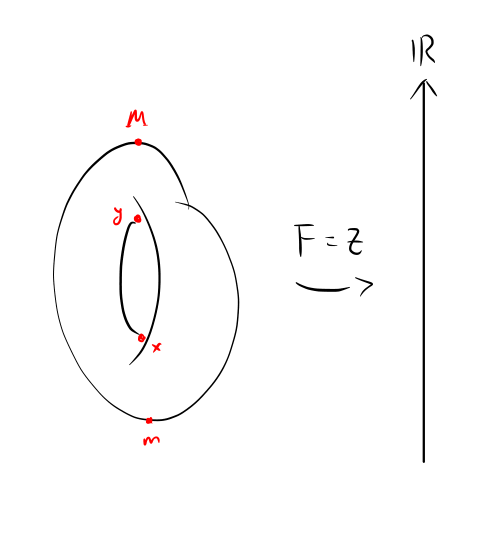
\includegraphics[scale=0.5]{sources/1.1}
\caption{העתקת גובה מהטורוס, והנקודות הקריטיות שלה.}
\label{1.1}
\end{figure}

באיור
\ref{1.1}
הנקודות המסומנות מאדום הן הנקודות הקריטיות של
$F$.
נסמן
\[\text{.} \mbb{T}^a \ceq \set{p \in \mbb{T}^2}{F\prs{p} < a}\]
\begin{itemize}
\item עבור
$a \leq F\prs{m}$
נקבל
$\mbb{T}^a = \ns$.
\item עבור
$F\prs{m} < a \leq F\prs{x}$
נקבל
$\mbb{T}^a \cong D^2$.
ראו איור
\ref{1.2}.

\begin{figure}
\centering
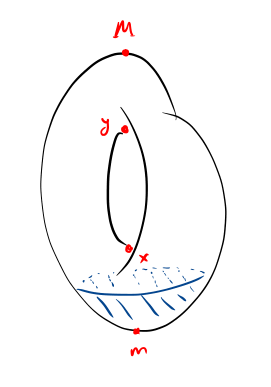
\includegraphics[scale=0.5]{sources/1.2}
\caption{חתך של הטורוס שדיפאומורפי ל־%
$D^2$.}
\label{1.2}
\end{figure}

\item עבור
$F\prs{x} < a \leq F\prs{y}$
נקבל
$\mbb{T}^a \cong S^1 \times \prs{0,1}$.
ראו איור

\begin{figure}
\centering
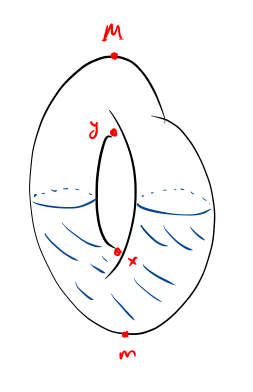
\includegraphics[scale=0.5]{sources/1.3}
\caption{חתך של הטורוס שדיפאומורפי ל־%
$S^1 \times \prs{0,1}$.}
\label{1.3}
\end{figure}

\item
עבור
$F\prs{y} < a \leq F\prs{M}$
נקבל
$\mbb{T}^a \cong \mbb{T}^2 \setminus D^2$.
\item עבור
$F\prs{M} < a$
נקבל
$\mbb{T}^a = \mbb{T}^2$.
\end{itemize}

\begin{corollary}
אם ב־%
$\left[ a, b \right)$
אין ערכים קריטיים אז
$\mbb{T}^a \cong \mbb{T}^b$.
\end{corollary}

נשאל איך משתנה הטופולוגיה במעבר בנקודות הקריטיות.
\begin{itemize}
\item במעבר דרך
$F\prs{m}$
יש הוספת דיסק.
\item כאשר
$a = x-\eps$
עבור
$\eps$
מספיק קטן, קו הגובה יראה באיור
\ref{1.4}
אם נדביק את
$\mbb{T}^a$
על פס כבאיור
\ref{1.5}
נקבל יריעה דיפאומורפית ל־%
$\mbb{T}^x+\eps$.

\begin{figure}
\centering
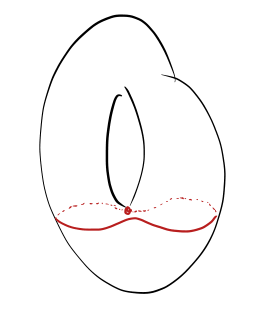
\includegraphics[scale=0.5]{sources/1.4}
\caption{קו גובה על הטורוס קרוב לנקודת אוכף.}
\label{1.4}
\end{figure}

\begin{figure}
\centering
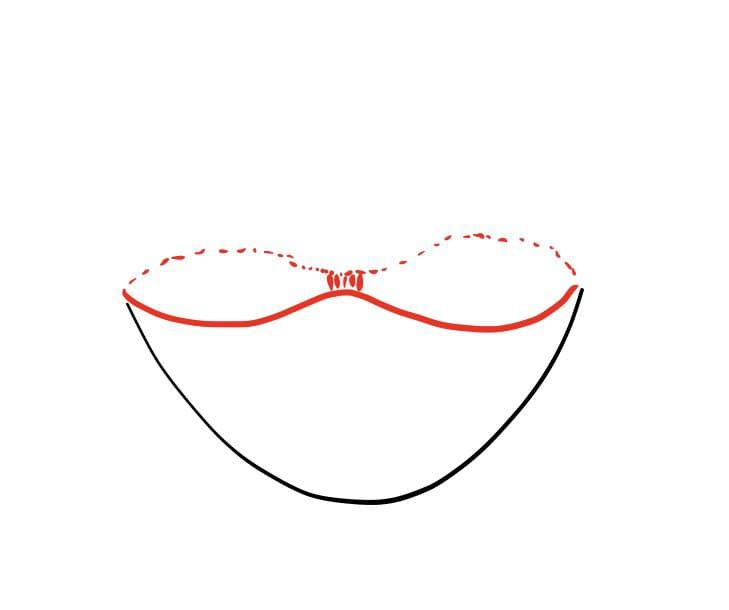
\includegraphics[scale=0.3]{sources/1.5}
\caption{הדבקת חתך של הטורוס קרוב לנקודת אוכף.}
\label{1.5}
\end{figure}

\item כאשר
$a = y+\eps$
עבור
$\eps$
מספיק קטן נקבל כי
$\mbb{T}^a$
כבאיור
\ref{1.6}.
אם נדביק את העיגולים באידומים באיור על פס כבאיור
\ref{1.7}
נקבל יריעה דיפאומורפית ל־%
$\mbb{T}^a$
עבור
$a = y + \eps$.

\begin{figure}
\centering
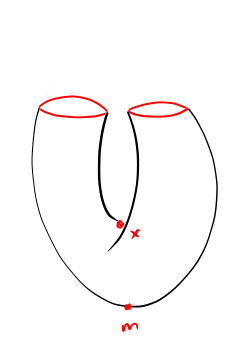
\includegraphics[scale=0.5]{sources/1.6}
\caption{חתך של הטורוס קרוב לנקודת אוכף.}
\label{1.6}
\end{figure}

\begin{figure}
\centering
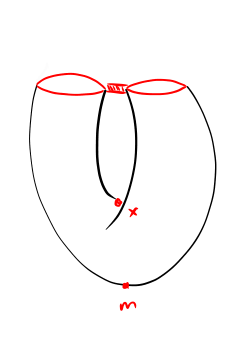
\includegraphics[scale=0.5]{sources/1.7}
\caption{הדבקת חתך של הטורוס קרוב לנקודת אוכף.}
\label{1.7}
\end{figure}

\item במעבר דרך
$F\prs{M}$
יש הדבקה של
$D^2$
לשפה של
$\mbb{T}^{F\prs{M} - \eps}$.
\end{itemize}

\end{example}

ראינו שבמקרה של הטורוס יש לנקודות הקריטיות חשיבות רבה במבנה של היריעה. אנחנו נראה בקורס שאפשר לשחזר אינווריאנטים כמו ההומולוגיה של יריעה בעזרת הבנה של הנקודות הקריטיות.
במקרה של הטורוס, מתקיים
\begin{align*}
H_0\prs{\mbb{T}^2, \mbb{Z}} &= \mbb{Z} \cong \mbb{Z}\trs{m} \\
H_1\prs{\mbb{T}^2, \mbb{Z}} &= \mbb{Z}^2 \cong \mbb{Z}\trs{x,y} \\
\text{.} H_2\prs{\mbb{T}^2, \mbb{Z}} &= \mbb{Z} \cong \mbb{Z}\trs{M}
\end{align*}
נדבר על דרך כללית להבין הומולוגיה וקוהומולוגיה של יריעות בעזרת נקודות קריטיות. נדבר על דואליות פואנקרה, על מבנה של כפל בקוהומולוגיה, על העתקות טבעיות, על מקדמים בחוגים שונים, וכו'.

בין היתרונות של תורת מורס הם שהיא נותנת את ה(קו)הומולוגיות הסטנדרטיות על יריעות, ושהיא עובדת עבור אוביקטים אינסוף־מימדיים.

\begin{example}[\textenglish{Path-Space}]
תהי
$M$
יריעה רימנית ויהי
\[\text{.} \mcal{P}\prs{x,y} = \set{\gamma \colon \brs{0,1} \to M}{\substack{\gamma\prs{0} = x \\ \gamma\prs{1} = y}}\]
על מרחב זה אפשר להגדיר כל מני פונקציות, למשל
\begin{align*}
\len \colon \mcal{P}\prs{x,y} &\to \mbb{R} \\
\text{.} \gamma &\mapsto \int_0^1 \norm{\dot{\gamma}} \diff s
\end{align*}

אפשר לנסות לעבוד עם תורת מורס על פונקציה כזאת ולהבין את המרחב
$\mcal{P}\prs{x,y}$
בעזרת הנקודות הקריטיות של
$\len$.
במקרה הזה, הנקודות הקריטיות הן קווים גיאודזיים. הן אינן מבודדות וקשה להסיק דברים על המרחב.

במקרה של
\[ \phi\prs{\gamma} = \int_0^1 \norm{\dot{\gamma}}^2 \diff s\]
הנקודות הקריטיות יהיו קווים גיאודזים עם מהירות קבועה. אז הנקודות הקריטיות בדרך כלל יהיו מבודדות, ויהיה אפשר להשתמש בתורת מורס.
\end{example}

\section{נקודות קריטיות}

במהלך הקורס נניח כי כל המבנים חלקים.
התוצאות נכונות באופן כללי יותר עבור יריעות
$\mcal{C}^2$,
שדות וקטוריים
$\mcal{C}^1$
ופונקציות דיפרנציאביליות
$\mcal{C}^2$.

\begin{definition}[נקודה קריטית]
תהי
$F \colon M \to N$
העתקה חלקה בין יריעות חלקות.
נקודה
$p \in M$
נקראת
\emph{קריטית}
אם
$D f_p \colon T_p M \to T_{f\prs{p}} N$
אינה על.
\end{definition}

\begin{remark}
\begin{enumerate}
\item במסגרת הקורס נדון בפונקציות
$F \colon M \to \mbb{R}$.
אז
$p \in M$
נקודה קריטית אם ורק אם
\[D F_p \colon T_p M \to T_{f\prs{p}} \mbb{R}\]
אינה על.
כיוון ש־%
$T_{f\prs{p}} \mbb{R}$
מרחב לינארי חד־מימדי זה שקול לכך שמתקיים
$D F_p = 0$.

\item
ניתן לזהות
$T_{f\prs{p}}\mbb{R} \cong \mbb{R}$
בדרך קנונית. נגדיר את ההרכבה של העתקה זאת על
$D F_p$
להיות
\emph{הנגזרת החיצונית של
$F$
בנקודה
$p$}.
נראה זאת בדיאגרמה הבאה.
\[
\begin{tikzcd}
T_p M \arrow[r, "D F_p"] \arrow[dr, dotted, swap, "\diff F_p"] & T_{f\prs{p}}\prs{\mbb{R}} \arrow[d, "\sim" labl] \\ & \mbb{R}
\end{tikzcd}
\]
נקבל כי
$p \in M$
נקודה קריטית אם ורק אם
$\diff F_p = 0$.

זאת תהיה ההגדרה שנעבוד איתה במשך רוב הקורס.

\item אם נפתח את ההגדרה של הנגזרת החיצונית נקבל כי
$p \in M$
נקודה קריטית אם ורק אם
$\frac{\del F}{\del v}\prs{0} \ceq \diff F_p\prs{v} = 0$
לכל
$v \in T_p M$.
מכך נסיק כי נקודות מינימום ומקסימום הן נקודות קריטיות.
כמו כן, ניתן לראות מכך כי נקודות אוכף הן נקודות קריטיות.
\end{enumerate}
\end{remark}

\begin{example}
יהי
$M \subseteq \mbb{R}^3$
משטח ותהי
$F \colon M \to \mbb{R}$
פונקציית גובה.
נגדיר
\begin{align*}
f \colon \mbb{R}^3 &\to \mbb{R} \\
\pmat{x\\y\\z} &\mapsto z
\end{align*}
ואז
$F = \rest{f}{M}$.

אז
$\diff f = \diff z$
ומתקיים
\[\text{.} \diff F_p = \rest{\diff f}{T_p M} = \rest{\diff z}{T_p M}\]
אז
\begin{align*}
\diff F_p = 0 &\iff \rest{\diff z}{T_p M} = 0
\\&\iff T_p M = \ker\prs{\diff z}
\\&\iff T_p M \parallel \spn\prs{x,y} \\
\\&\iff T_p M = \pmat{0 \\ 0 \\ 1}^\perp \\
\\\text{.} \hphantom{\diff F_p = 0} T_p M^\perp = \span\set{\pmat{0\\0\\1}}
\end{align*}
בדוגמה באיור
\ref{1.1}
נקבל שהנקודות הקריטיות הן בדיוק אלו המסומנות. אלו הנקודות בהן הנורמל למישור הוא כפולה של
$z$.
\end{example}

כעת נרצה לעבוד עם שדות וקטוריים במקום נגזרות חיצוניות. במקרה זה אפשר להסתכל על זרימות לאורך שדה ועל הומוטופיות, מה שחסר במקרה של הנגזרת חהיצונית. נתחיל בהגדרה של גרדיאנט ובקשר שלו לנגזרת החיצונית.

\begin{definition}[גרדיאנט]
תהי
$\prs{M,g}$
יריעה רימנית.
ותהי
$F \colon M \to \mbb{R}$
פונקציה חלקה.
לכל
$p \in M$,
$g$
משרה איזומורפיזם
\begin{align*}
g \colon T_p M &\riso T_p^* M \\
\text{.} \hphantom{lalala} v &\mapsto g\prs{v, \cdot}
\end{align*}

\emph{הגרדיאנט של
$F$}
שנסמנו
$\nabla_g F$
או בדרך כלל
$\nabla F$
מוגדר להיות השדה היחיד המקיים
\begin{align*}
\text{.} g\prs{\nabla F, \cdot} = \diff F
\end{align*}
\end{definition}

\begin{remark}
הגרדיאנט
$\nabla F$
תלוי בבחירת
$g$!
\end{remark}

\begin{remark}
מתקיים
\[\diff F_p = 0 \iff \nabla_g F_{\prs{p}} = 0\]
וזה בלתי־תלוי בבחירת
$g$.

נקבל מכך כי
$p \in M$
נקודה קריטית עבור
$F$
אם ורק אם
$\nabla F_{\prs{p}} = 0$.
\end{remark}

\begin{proposition}
תהי
$F \colon M \to \mbb{R}$
ויהיו
$a < b$
כך שקיים
$\eps > 0$
עבורו הקטע
$\prs{a-\eps, b}$
אינו מכיל ערכים קריטיים.
לדוגמא ראו איור
\ref{1.8}.

\begin{figure}
\centering
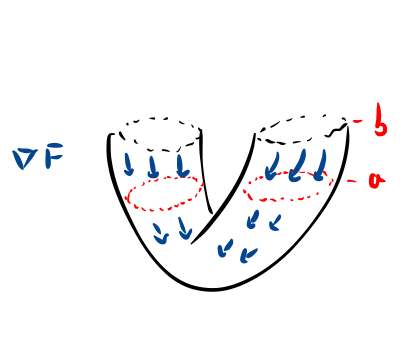
\includegraphics[scale=0.5]{sources/1.8}
\caption{זרימה על הטורוס לאורך הגרדיאנט.}
\label{1.8}
\end{figure}

אז יש דיפאומורפיזם
$M^a \cong M^b$.
\end{proposition}

\begin{proof}
נרצה לנרמל את הגרדיאנט כדי שמהירות הזרימה תהיה אחידה. כדי לא לחלק באפס, נאפס את השדה מתחת לגובה
$a-\eps$.

תהי
$g$
מטריקה רימנית על
$M$.
נסמן
$X = -\nabla_g F$.
עבור
$p \in M^b$
נסתכל על
$\frac{X_p}{\norm{X_p}^2}$.
זה מגדיר שדה וקטורי שלאורכו
$F$
יורדת במהירות
$1$.%
\footnote{
גיאומטרית,
$\frac{X}{\norm{X}}$
וקטור יחידה שמצביע בכיוון בו
$F$
עולה הכי מהר, ומהירות העליה לאורכו היא
$\norm{X}$. לכן כדי שהמהירות תהיה קבועה חלקנו ב־%
$\norm{X_p}^2$.}
%TODO footnote ruler to the right

תהי
\begin{align*}
\rho \colon \prs{-\infty, b} \to \mbb{R}
\end{align*}
חלקה עבורה
\begin{align*}
\rest{\rho}{-\infty, a-\eps} &\equiv 0 \\
\rest{\rho}{\prs{a,b}} &\equiv 1 \\
\text{.} \hphantom{lala} \rho' \geq 0
\end{align*}
אז נוכל להגדיר
\[X' = \frac{\rho X_p}{\norm{X_p}^2}\]
לכל
$F\prs{p} \in \prs{a-\eps, b}$
ונרחיב את
$X'$
מתחת לגובה
$a-\eps$
עם אפסים.
למד"ר המוגדרת על ידי
$X'$
יש פתרונות לכל זמן
$t \geq 0$.

תהי
$\phi_t \colon M^b \to M^b$
זרימה של
$X'$.
אז
$\phi_{b-a} \colon M^b \riso M^a$
דיפאומורפיזם.
\end{proof}

\section{הדבקת ידיות}

\subsection{פונקציות מורס}

נרצה כעת להבין מה קורה איך היריעות
$M^a, M^b$
משתנות כאשר עברו מ־%
$a$
ל־%
$b$
דרך נקודה קריטית.
זה דבר מסובך מאוד באופן כללי ולכן ניאלץ לצמצם את הדיון לנקודות קריטיות שאינן מנוונות.

\begin{definition}[הסיאן]
תהי
$M$
יריעה רימנית ותהי
$F \colon M \to \mbb{R}$
חלקה.
לכל
$p \in $
נגדיר
\[\mrm{Hess}_p\prs{F} \colon T_p M \times T_p M \to \mbb{R}\]
על ידי
$\mrm{Hess}\prs{F} = \nabla \diff F$
כאשר
$\nabla$
הוא ה־%
\href{https://en.wikipedia.org/wiki/Levi-Civita_connection}{\textenglish{Levi-Civita Connection}}.

הגדרה מפורשת יותר היא
\begin{align*}
\mrm{Hess}_p\prs{F} \prs{X_p,Y_p} &= \trs{\nabla_X \mrm{grad}\prs{F_p}, Y_p}
\\&= L_X L_Y \prs{F} - \diff F_p\prs{\nabla_X Y}
\end{align*}
עבור שני שדות וקטוריים
$X,Y$
שמוגדרים סביב
$p$.
\end{definition}

\begin{remark}
הבחירה של ההסיאן תלויה בבחירה של המטריקה הרימנית.

במקרה הפרטי ש־%
$p$
נקודה קריטית מתקיים
$\diff F_p = 0$
ואז
\[\text{.} \mrm{Hess}_p\prs{F}\prs{X_p, Y_p} = L_X L_Y\prs{F}\]
בפרט, הערך של ההסיאן בנקודה הקריטית אינו תלוי בבחירה של המטריקה הרימנית.
\end{remark}

\begin{remark}
אם
$p$
נקודה קריטית של
$F$
נוכל להגדיר את ההסיאן כהעתקה
$T_p M \times T_p M \to \mbb{R}$
באופן הבא.
יהיו
$X,Y \in T_p M$.
נרחיב את
$X,Y$
לשדות לוקליים
$\tilde{X}, \tilde{Y}$
סביב
$p$.
אז
\[\text{.} \mrm{Hess}_p\prs{F} \prs{X,Y} \ceq L_{\tilde{X}} L_{\tilde{Y}}\prs{F}\prs{p}\]
\end{remark}

\begin{definition}[נגזרת לי]
עבור שדה וקטורי
$\tilde{Y}$
ונקודה
$p \in M$
נגדיר
\begin{align*}
L_{\tilde{Y}}\prs{F}\prs{p} &= \lim_{t\to 0} \frac{\prs{f\prs{\phi_{\tilde{Y}}^t\prs{p}} - f\prs{p}}}{t} \\&=
d F_p\prs{\tilde{Y}_p}
\\ &=
\frac{\del F}{\del \tilde{Y}}\prs{p}
\end{align*}
כאשר
$\phi_{\tilde{Y}}$
הזרימה לפי
$\tilde{Y}$.
\end{definition}

\begin{remark}
נקבל מההגדרה כי
\begin{align*}
\prs{L_{\tilde{X}} L_{\tilde{Y}}}\prs{p}
&=
\diff \prs{L_{\tilde{Y}} F}_p \prs{\tilde{X}_p}
\\&=
\diff \prs{L_{\tilde{Y}} F}_p \prs{X}
\end{align*}
ולכן
$\mrm{Hess}_p \prs{F}$
אינו תלוי בבחירת ההרחבה
$\tilde{X}$
של
$X$.
\end{remark}

נראה שההסיאן סימטרי ב־%
$X,Y$
ונקבל מכך כי ההסיאן אינו תלוי בבחירת ההרחבה
$\tilde{Y}$
של
$Y$.

\begin{proposition}
\[\text{.} \mrm{Hess}_p\prs{F}\prs{X,Y} = \mrm{Hess}_p\prs{F}\prs{Y,X}\]
\end{proposition}

\begin{proof}
מתקיים
\begin{align*}
\mrm{Hess}_p\prs{F}\prs{X,Y} - \mrm{Hess}_p\prs{F}\prs{Y,X}
&=
L_{\tilde{X}} L_{\tilde{Y}}\prs{F}_p - L_{\tilde{Y}}L_{\tilde{X}}\prs{F}_p
\\&=
L_{\brs{\tilde{X}, \tilde{Y}}} F_p
\\&= \cancelto{0}{\diff F_p} \prs{\brs{\tilde{X}, \tilde{Y}}_p}
\\ \text{.} \hphantom{\mrm{Hess}_p\prs{F}\prs{X,Y} - \mrm{Hess}_p\prs{F}\prs{Y,X}} &= 0 
\end{align*}
\end{proof}

\begin{corollary}
$\mrm{Hess}_p\prs{F}\prs{X,Y}$
אינה תלויה בבחירת ההרחבות
$\tilde{X}, \tilde{Y}$.
\end{corollary}

\begin{exercise}
בקואורדינטות מקומיות סביב
$p$
\begin{align*}
\hat{F} \colon \mbb{R}^n \to \mbb{R}
\end{align*}
מתקיים
\[\text{.} \mrm{Hess}_{\hat{p}}\prs{\hat{F}} \colon T_{\hat{p}} U \times T_{\hat{p}} U \to \mbb{R}\]
אם נזהה
$T_{\hat{p}}U \cong \mbb{R}$
נקבל העתקה
$\prs{\mbb{R}^n}^2 \to \mbb{R}$.
העתקה זאת מיוצגת על ידי המטריצה
\[\pmat{\frac{\del^2 \hat{F}}{\del x_i \del x_j}\prs{\hat{p}}}_{i,j \in [n]}\]
כמו בקורסי אינפי.
\end{exercise}

\begin{notation}
נסמן ב־%
$\mrm{Crit}\prs{F}$
את אוסף הנקודות הקריטיות של
$F$.
\end{notation}

\begin{definition}[נקודה קריטית לא־מנוונת]
$p \in \mrm{Crit}\prs{F}$
\emph{לא מנוונת
\textenglish{non-degenerate}}
אם
$\mrm{Hess}_p\prs{F}$
תבנית לא מנוונת (באופן שקול, אם
$\ker\prs{\mrm{Hess}_p} = \set{0}$,
ובאופן שקול אם
$0$
אינו ערך עצמי).
\end{definition}

\begin{example}
תהי
\[S^2 = \set{\prs{x,y,z} \in \mbb{R}^3}{x^2 + y^2 + z^2 = 1}\]
ותהי
\begin{align*}
F \colon S^2 &\to \mbb{R} \\
\text{.} \pmat{x\\y\\z} &\mapsto z
\end{align*}
תהי
$p = \pmat{0\\0\\1}$.
זאת נקודה קריטית כי הנורמל לספירה ב־%
$p$
מצביע למעלה.

נבחר קבוצה פתוחה
$U$
קטנה סביב
$p$,
ומפת קואורדינטות
\begin{align*}
\phi \colon U &\to \mbb{R}^2 \\
\text{.} \pmat{x\\y\\z} &\mapsto \pmat{x\\y}
\end{align*}
אז הצגה מקומית היא
\begin{align*}
\hat{F} \colon \phi\prs{U} &\to \mbb{R} \\
\pmat{x\\y} &\mapsto \sqrt{1-x^2 - y^2}
\end{align*}
ואז
\begin{align*}
\mrm{Hess}_0\prs{\hat{F}} &= \pmat{\frac{\del^2 \hat{F}}{\del x^2} \prs{0} & \frac{\del^2 \hat{F}}{\del x \del y} \prs{0} \\ \frac{\del^2 \hat{F}}{\del y \del x}\prs{0} & \frac{\del^2 \hat{F}}{\del y^2}\prs{0}} = \pmat{-1 & 0 \\ 0 & -1}
\end{align*}
לא מנוונת.

באופן דומה
\[\text{.} \mrm{Hess}_{\hat{s}}\prs{\hat{F}} = \pmat{1 & 0 \\ 0 & 1}\]
\end{example}

\begin{definition}[פונקציית מורס]
$F \colon M \to \mbb{R}$
חלקה היא
\emph{פונקציית מורס}
אם כל הנקודות הקריטיות שלה אינן מנוונות.
\end{definition}

\subsection{הלמה של מורס}

עבור
$F \colon M \to \mbb{R}$
נוכל לקחת פיתוח טיילור של הצגה מקומית של
$F$.

\begin{align*}
\hat{F}\prs{x+\Delta x} &= \hat{F}\prs{x} + \sum_{i \in [n]} \frac{\del \hat{F}}{\del x_i} \del x_i + \frac{1}{2} \sum_{i,j \in [n]} \frac{\del^2 \hat{F}}{\del x_i \del x_j} \Delta x_i \Delta x_j + O\prs{\norm{\Delta x}^3}
\\&=
\hat{F}\prs{x} + D \hat{F}\prs{\Delta x} + \mrm{Hess}_x\hat{F}\prs{\Delta x, \Delta x} + O\prs{\norm{\Delta x}^3}
\end{align*}

אם
$x$
נקודה קריטית לא־מנוונת של
$\hat{F}$
אז
\begin{align*}
\text{.} D \hat{F}\prs{\Delta x} = 0
\end{align*}
הלמה של מורס אומרת שבמקרה זה אפשר לבחור קואורדינטות סביב
$x$
עבורן
\[\text{.} O\prs{\norm{\Delta x}^3} = 0\]
זאת אומרת,
\[\text{.} \hat{F}\prs{x + \Delta x} = \hat{F}\prs{x} + \mrm{Hess}_x\prs{\hat{F}} \prs{\Delta x, \Delta x}\]
נפעיל את משפט סילבסטר כדי להביא את ההסיאן לצורה קנונית ונקבל מערכת קואורדינטות
$y$
לפיה
\begin{align*}
\text{.} \hat{F}\prs{y + \Delta y} = \hat{F}\prs{y} - \sum_{i \in [k]} y_i^2 + \sum_{i = k+1}^n y_i^2
\end{align*}

\begin{theorem}[הלמה של מורס]
תהי
$x \in Mn$
נקודה קריטית לא־מנוונת של
$F \colon M \to \mbb{R}$
חלקה.
קיימת מפת קואורדינטות
$\prs{U,\phi}$
סביב
$x$
כך שמתקיים
$\phi\prs{x} = 0$
ושעבור
\[\hat{F} = F \circ \phi^{-1} \colon \phi\prs{U} \to \mbb{R}\]
מתקיים
\begin{align*}
\text{.} \hat{F}\prs{y} = \hat{F}\prs{0} - \sum_{j \in [i]} y_j^2 + \sum_{j = i+1}^n y_j^2
\end{align*}
\end{theorem}

\begin{proof}
נבחר מפה כלשהי
$\prs{U,\psi}$
סביב
$x$.
בלי הגבלת הכלליות נניח כי
$\psi\prs{x} = 0$.
שינוי לינארי של הקואורדינטות משרה את אותו השינוי על
$T_p \mbb{R}^n$
לכל
$p \in \psi\prs{U}$.
כלומר, אם
\begin{align*}
f \colon \mbb{R}^n \to \mbb{R}^n \\
y &\mapsto A y
\end{align*}
לינארית עבור
$A \in M_n\prs{\mbb{R}}$
אז
\begin{align*}
D f_p \colon T_p \mbb{R}^n &\to T_p \mbb{R}^n \\
\text{.} \hphantom{lalalalala} v &\mapsto A v
\end{align*}
לפי משפט סילבסטר קיימת מטריצה מעבר
$A \in M_n\prs{\mbb{R}}$
שמלכסנת את
$\mrm{Hess}_0\prs{\hat{F}}$.
אם נפעיל על
$\psi\prs{U}$
החלפת קואורדינטות
$y \mapsto Ay$
נקבל מפה חדשה
$\prs{U, A \cdot \psi}$
עבורה
$A \cdot \psi\prs{x} = 0$
וגם
\[\mrm{Hess}_0\prs{\hat{F}}\]
מטריצה אלכסונית ללא אפסים ע האלכסון, כאשר
$\hat{F}$
הצגה של
$F$
לפי
$A \cdot \psi$.
מכאן, נניח בלי הגבלת הכלליות שבחרנו מפה
$\psi$
לפיה
$\mrm{Hess}_0\prs{\hat{F}}$
אלכסונית.

נמשיך את ההוכחה באינדוקציה על המימד.

\begin{description}
\item[בסיס, $n = 1$:]
נסתכל על הצגה מקומית
\begin{align*}
\hat{F}\prs{y} &= \hat{F}\prs{0} + \frac{1}{2} \hat{F}''\prs{0} y^2 + r\prs{y}
\end{align*}
עבור
$r\prs{y} \in O\prs{\norm{y}^3}$.
אנו יודעים כי
$r\prs{y}$
פונקיה חלקה כצירוף פונקציות חלקות.
כיוון ששתי הנגזרות הראשונות שלה מתאפסות ב־%
$0$
נקבל כי גם
$\frac{r\prs{y}}{y^2}$
פונקציה חלקה.
אז נוכל לכתוב
\begin{align*}
\hat{F}\prs{y} = \hat{F}\prs{0} \pm K y^2 \prs{1 + \eps\prs{y}}
\end{align*}
כאשר
\[K = \abs{\frac{1}{2} \hat{F}''\prs{0}} > 0\]
וכאשר
\[\text{.} \eps\prs{y} = \frac{r\prs{y}}{y^2 K} \xrightarrow{y\to 0} 0\]
נגדיר
\[\text{.} y_1 = \Theta\prs{y} \ceq y \sqrt{K\prs{1+\eps\prs{y}}}\]
אז
$\Theta \colon y \to y_1$
מוגדרת היטב סביב
$y = 0$,
וגם
$\Theta'\prs{0} = \sqrt{K} \neq 0$.
לכן
$\Theta$
דיפאומורפיזם מקומי סביב
$y = 0$.
נקבל כי
\begin{align*}
\hat{F} \circ \Theta^{-1}\prs{y_1} &= \hat{F}\prs{y}
\\&=
\hat{F}\prs{0} \pm K y^2 \prs{1 + \eps\prs{y}}
\\&=
\hat{F}\prs{0} \pm y_1^2
\end{align*}
וזאת הצורה הרצויה.

\item[צעד:]
אחרי פסח...
%TODO
\end{description}
\end{proof}

%TODO

\backmatter
\end{document}